\subsection{Grading based on Inlinks and Outlinks} % eller: Grading based on inlink and outlinks 
\label{sec:grading_based_on_inlinks_and_outlinks}
Our first assumption is that categories with high a inlink number (number of categories linking to a category) can be reached from categories with unrelated topics. An example of a category with a high inlink number is  \emph{World War II}. This category can be reached from 87 different categories (see figure \ref{fig:high_inlink_number}). 


\begin{figure}[h]
\centering
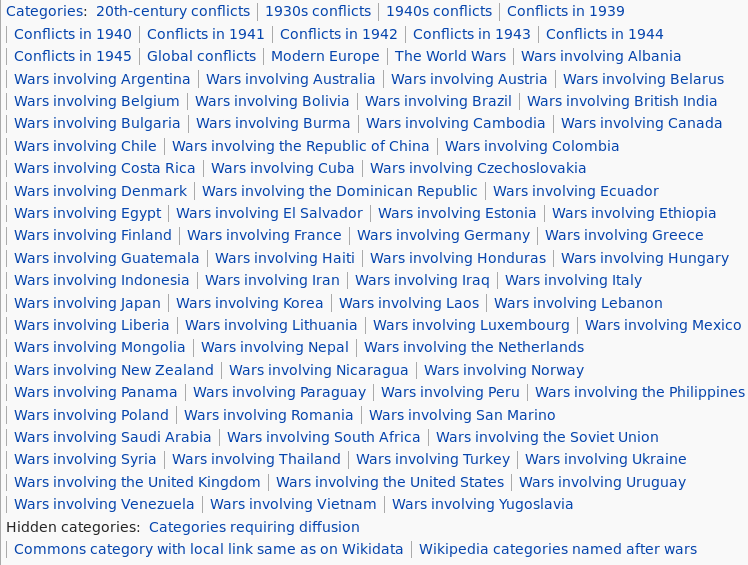
\includegraphics[width=\textwidth]{Chapters/Implementation/Grading/high_inlink_number}
\caption[Example of category with high \emph{inlink number}]{All categories linking to the category \emph{World War II}. This is an example of a category with high inlink number.}
\label{fig:high_inlink_number}
\end{figure}


\begin{comment}
\begin{figure}[h]
\centering
\begin{lstlisting}
ole-johan dahl:
*politics/political activism/leadership/management/quality/software quality/formal methods/formal methods people
\end{lstlisting}
\caption{Example of how \emph{politics} can reach the article about \emph{Ole-Johan Dahl}}
\label{fig:politicstosoftware}
\end{figure}
\end{comment}

The next assumption is that categories with a high outlink number (number of categories reached from a category) are more likely to reach categories not relevant since they can reach far in all the subcategories' directions. Figure \ref{fig:high_outlink_number} illustrates number of subcategories found for the category with highest outlink number, which is the category \emph{Albums by artist} with a outlink number of 17 393. 


\begin{figure}[h]
\centering
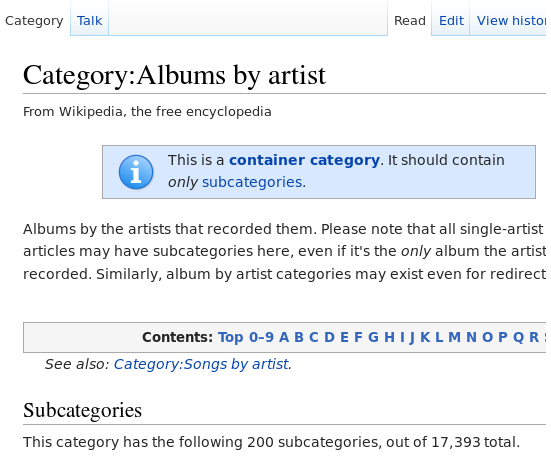
\includegraphics[width=0.7\textwidth]{Chapters/Implementation/Grading/high_outlink_number}
\caption[Example of category with high \emph{outlink number}]{The category \emph{Albums by artist} is an example of category with high outlink number. }
\label{fig:high_outlink_number}
\end{figure}


These assumption combined are the foundation of grading based on inlink and oulink numbers. Categories frequently reached should obtain a lower score than categories rarely reached. We need some way of deciding whether an inlink number is high for each category. This can be done by comparing the inlink number with the average inlink number, and similarly for outlink number and the average outlink number. 


The average inlink and outlink numbers are found by summarizing all inlink numbers and outlink number respectively, and dividing the result on number of categories. Table \ref{tab:avginlinkoutlink} shows the results found. 


\begin{table}[ht]
\centering
\renewcommand{\arraystretch}{1.25}
\begin{tabular}{c |c}
\textbf{Average \emph{inlink number}} & \textbf{Average \emph{outlink number}}\\ \hline
 5 & 2 
\end{tabular}
\\[10pt]
\caption{Average inlink number and outlink number for all categories.}
\label{tab:avginlinkoutlink}
\end{table}
The score for each category was found with equation \ref{eq:categoryscore}, where each category's inlink number and outlink number is compared by the average inlink and outlink number.

%The scoring from formula \ref{eq:scoreinout} means that paths with categories rarely visited will be favoured, hence given a lower score. 

\subsubsection{Evaluation of the scores}
None of the categories can have a score of 0 since all Wikipedia categories are connected to at least one other category \footnote{We mentioned in challenges (Introduction, encoding) that some of our connections were broken. This does not affect the scoring of the categories, since the inlink and outlink numbers are preserved for all categories. }. The lowest score found was 0.376010, which was given to all categories with only one parent category and with none subcategories. This was a total of 104 471 categories.  The category with the highest score is the category \emph{Albums by Artist}, which is the category with most subcategories (17 393), hence a score of $6 512.120784$. The range of the scores is \emph{<0.376010, 6 512.120784>}, which means that all scores is within this range. 

The figures in \ref{fig:score_values} shows the number categories found for each of the possible score values. Figure \ref{fig:scorevalue}) illustrates the results for all possible score values, while figure \ref{fig:25_smallest}) illustrates the  25 smallest sore values and their corresponding number of categories. These figures shows that there are many categories with low score values, while there are only a few categories for higher score values. The categories with high score value will have a high impact on the article path, which means that paths containing these categories will have a lower probability of be considered relevant. 


\begin{figure}[h]
\centering
\begin{subfigure}[b]{\textwidth}
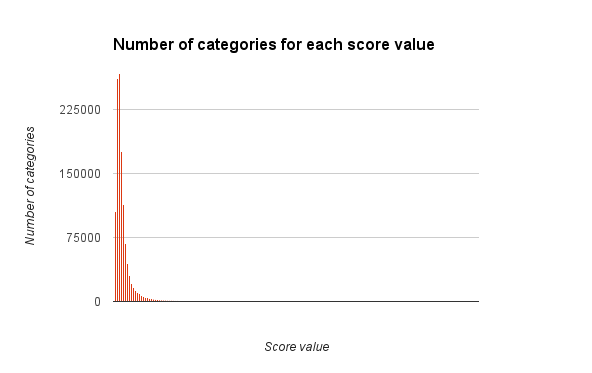
\includegraphics[width=\textwidth]{Chapters/Implementation/Grading/Inlinkoutlink_scorevalue_numberofcategories}
\caption{Number of categories for each possible score value.}
\label{fig:scorevalue}
\end{subfigure}
%\begin{figure}[h]
%\centering
\begin{subfigure}[b]{\textwidth}
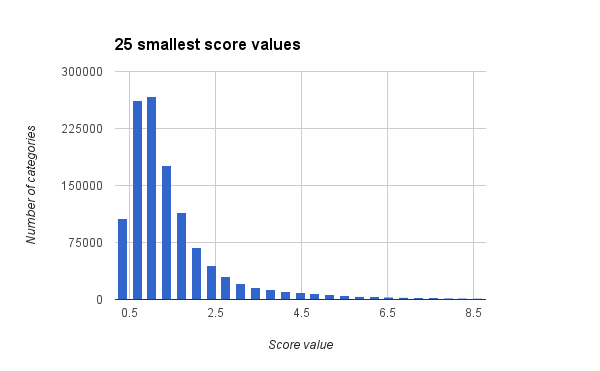
\includegraphics[width=\textwidth]{Chapters/Implementation/Grading/25_smalles_score_values}
\caption{The 25 smallest score values and their corresponding number of categories. These are the most common score values since they are connected to categories with low inlink and outlink numbers.}
\label{fig:25_smallest}
\end{subfigure}
\caption{Number of categories for available score value. }
\label{fig:score_values}
\end{figure}

%This means that the score for all categories are between 0.376010 and 6512.120784.

%This means that the scores for all categories are in the range of 0 and

%Maxgrade: 6512.120784 (albums by artist)
%Mingrade: 0.376010 (user bho-4)
\subsection{Problems with the simplified grader}
Since it is desirable with the lowest score as possible, the first problem encountered was that the program favoured short paths. 

\begin{figure}
\centering
\begin{lstlisting}
argentines of serb descent:
* society/ethnicity/ethnicity stubs/ (34.592939)
* culture/ethnicity/ethnicity stubs/ (29.704807)
* humans/ethnic groups/ethnology/ethnicity stubs/ (27.824755)
\end{lstlisting}
\caption{Caption}
\label{fig:my_label}
\end{figure}

This is both correct and wrong at the same time. It is desirable to find short paths, but there should be some punishment if the path is too short?

\begin{comment}
Problem med Alexander Huges: han er fotballspiller og dette kommer ikke så godt fra. 

asd.,kas.kdfj
\end{comment}


\begin{figure}[h]
\centering
\begin{lstlisting}
alexander hughes:
*health/health by city/health in edinburgh/sport in edinburgh/sports teams in edinburgh/football clubs in edinburgh/heart of midlothian f.c./heart of midlothian f.c. players (37.22501)
*nature/life/births by year/year of birth missing (28.576777)
*people/people categories by parameter/people by time/births by year/year of birth missing (28.200766)
\end{lstlisting}

\caption{Caption}
\label{fig:alexanderhughes}
\end{figure}

